\documentclass[11pt]{IEEEtran}
\usepackage[brazilian]{babel}
\usepackage[utf8]{inputenc}
\usepackage[T1]{fontenc}
\usepackage{float}
\usepackage{graphicx}
\usepackage{caption}

\captionsetup[table]{skip=10pt}

\sloppy

\title{Programação Paralela\\ Trabalho II}

\author{Giovanni Cupertino, Matthias Nunes, \IEEEmembership{Usuário pp12820}}

\begin{document}

\maketitle

\section{Introdução}



\section{Análise dos Resultados Obtidos}

	\begin{table}[H]
		\centering
		%\scalebox{0.8}{
			\begin{tabular}{c|r|r|r|r}
				Processos & Normal & Otimizado & Normal O3 & Otimizado O3 \\
				\hline
				3  & 11,197245s & 5,030874s & 2,494979s & 1,122686s \\
				\hline
				7  &  2,864694s & 0,924965s & 0,639917s & 0,221029s \\
				\hline
				15 &  0,911735s & 0,360175s & 0,229385s & 0,080532s \\
				\hline
				31 &  0,379110s & 0,115022s & 0,077629s & 0,042855s \\
			\end{tabular}
		%}
		\caption{Resultados obtidos para 100000}
		\label{result_table}
	\end{table}

	\begin{table}[H]
		\centering
		%\scalebox{0.8}{
			\begin{tabular}{c|r|r|r|r}
				Processos & Normal & Otimizado & Normal O3 & Otimizado O3 \\
				\hline
				3  & 1118,725370s & 504,497851s & 260,702105s & 116,810162s \\
				\hline
				7  &  283,095140s &  92,283123s &  65,604866s & 21,520253s \\
				\hline
				15 &   73,926856s &  21,100409s &  16,904703s & 4,794249s \\
				\hline
				31 &   36,979798s &   9,868190s &   6,390105s & 1,807969s \\
			\end{tabular}
		%}
		\caption{Resultados obtidos para 1000000}
		\label{result_table}
	\end{table}

	%\begin{figure}[H]
		%\centering
		%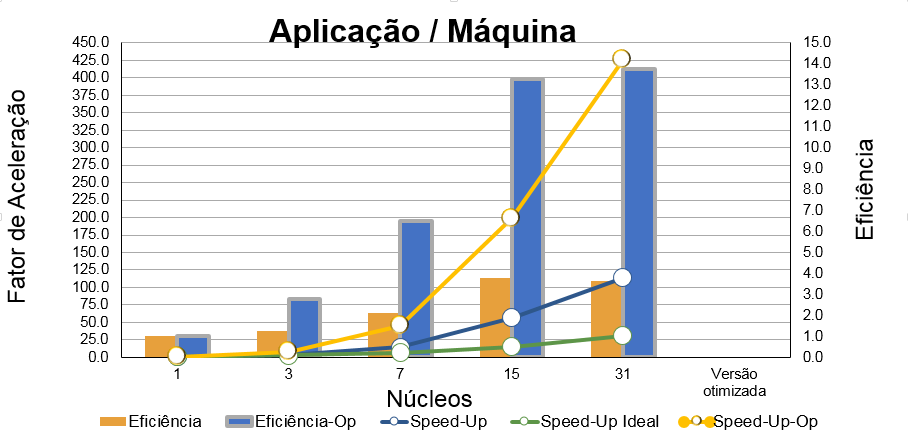
\includegraphics[width=88mm]{doc/graph.png}
		%\caption{Gráfico gerado a partir da tabela}
		%\label{fig_graph}
	%\end{figure}

\section{Dificuldades Encontradas}

	Não foram encontradas dificuldades na implementação desse trabalho, nem na
	utilização da biblioteca MPI\@.

\end{document}

